\chapter{绪论}
本章首先介绍社交多媒体数据的含义以及对于社交多媒体数据的研究意义,
并由此引出社交多媒体数据的研究中存在的关键问题。然后介绍本文的主要工作及创新点,
最后介绍全文的结构安排。

\section{社交多媒体数据研究意义}
近几年来,智能手机及其他智能移动设备呈现出了爆发式的增长与普及。
高清摄像头,大容量存储, 和高速的网络连接为用户创造了极其便利的拍摄条件,
从而创造了海量的个人多媒体数据。用户几乎可以在任何时间任何地点拍摄图片或者视频,
并将它们分享到社交网络或存储到云端服务器。
据统计, 截止到2014年产生了大约$2.7$万亿的用户图片。
到2017年,该数字将会增长到约$4.9$万亿~\cite{phototrend}。
这类由个人用户产生的多媒体数据具有明显的社交性特点:
\begin{enumerate}
    \item 用户通常在社交活动中拍摄视频或者图片, 同一时间段内其他用户也会拍摄与之相关的内容;
    \item 大量的个人多媒体数据被用户分享到Flickr,Instagram,YouTube,美拍,优酷等社交网站,
        这些数据本身包含的时间、地点等信息与其他用户分享的个人多媒体数据产生关联。
\end{enumerate}
因此,本文将这类用户数据统称为\textbf{社交多媒体数据}。

相比于传统的多媒体数据,个人用户产生的多媒体数据具有以下特点:
\begin{enumerate}
    \item \textbf{质量不确定}:由于个人用户拍摄技巧比较业余,
        拍摄时的光线限制,相机的快速移动或者抖动,场景快速变换等原因,
        个人多媒体数据通常伴有抖动,散焦,过度曝光/欠曝光,模糊,遮挡以
        及拍摄出无意义的视频或图片等问题,影响到个人多媒体数据的后期浏览体验。

    \item \textbf{内容冗余}:用户在拍照时通常采取多次拍摄的方式来获得最理想的拍照效果。
        一般情况下,用户会在短时间内选择最好的照片或视频分享到社交网络,
        却很少删除其他内容非常相似的数据,使得个人多媒体数据中有大量的冗余。
        这些冗余数据带来三个方面的主要问题:1)需要耗费大量的时间和精力去整理;
        2)占据了大量的存储资源; 3)增加了用户查找数据的难度。

    \item \textbf{多样性}:用户拍摄的时间、地点和环境比较随机,拍摄的角度,
        内容具有很大的不确定性,使得个人多媒体数据的内容表现出多样化的特点。
        个人多媒体数据相关的服务,不仅需要去除冗余的用户数据,同时也需要最大程度的保留用户数据的多样性。

    \item \textbf{故事性}:用户的拍摄行为并不是完全随机的,而是选择性地记录对于他们有意义的时刻和场景。
        相同时间段内相近地点拍摄的个人多媒体数据,浓缩了用户在一段时间内的足迹,以及经历的活动。
        而完整的个人多媒体数据则记录了很长一段时间内发生在用户身上的故事。
        然而,当前的个人多媒体数据服务还不能很好的将这些记录的原始片段,整理成高观赏性的纪录片。

    \item \textbf{具有位置和时间信息}:现代移动设备拍摄时一般都能检测到拍摄的时间、地点等信息,
        并将这些信息存储在图像或者视频的文件头中。这些时间和地点信息记录了拍摄时的时空上下文关系,
        使得数据之间能够产生关联。基于用户历史拍摄的时间、地点和具体内容,可以更好的挖掘出
        发生在用户身上的故事。
\end{enumerate}

\begin{figure}[ht]
\centering
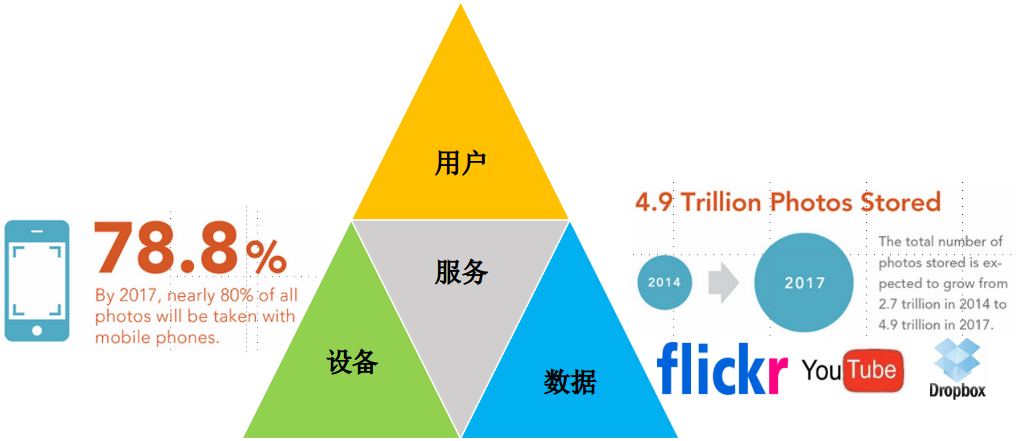
\includegraphics[width=0.9\textwidth]{social-media.png}
\caption{社交多媒体数据的产生和利用现状} \label{fig:status}
\end{figure}
然而,由于缺乏智能的社交多媒体数据建模和表达服务,这些海量的数据所包含的信息并没有得到
充分的挖掘和利用。如图~\ref{fig:status}所示,一方面,社交多媒体数据呈现出并保持着爆炸式的增长趋势;
另一方面,这些记录了珍贵记忆的用户数据被大量的存在本地或者云端磁盘上,
却很少再次被用户浏览。社交多媒体数据中所蕴含的故事性和社交性,并没有带来更好的用户体验。
随着人们对于多媒体内容品质和个性化需求的提高,越来越多的研究人员和工业界研究机
构投入更多的精力到社交多媒体数据中。
此外,由于社交多媒体数据的数量庞大,质量不确定、内容冗余、多样,
并带有丰富的社交信息,对相关的处理算法提出了更复杂的要求。
因此,对于社交多媒体数据的研究已成为计算机视觉领域的研究热点,相关的成果既有利于
推动计算机视觉以及多媒体领域相关课题的创新,
对于用户体验的提升以及工业界的发展都也具有重要的应用价值和现实意义。

\section{社交多媒体数据关键问题}
\label{sec:key_problems}
社交多媒体数据的研究涉及内容的语义理解以及应用层的关联表达两个大的方面。
其中,语义理解面临的主要问题包括:
\begin{itemize}
    \item 解决标注难的问题。机器学习算法可以归纳为有监督学习,
        半监督学习,和无监督学习三个类别。
        有监督学习通常能够获得最好的分类效果。然而,它依赖大量准确的标注数据,
        在当前大数据的背景下有监督学习的应用成本十分高昂。
        据了解,目前最大的有标注图片数据集ImageNet~\cite{russakovsky2015imagenet}
        花费了大约$25,000$名用户一年左右的时间完成标注。
        尽管如此,ImageNet仅包含$22,000$个类别,与现实应用中的语料库相差甚远(如WordNet
        ~\footnote{\url{http://wordnet.princeton.edu/}})。
        与之相反,半监督学习和无监督的学习不需要大量的标注,但是分类的效果与有监督学习
        还有明显的差距。 基于以上问题,
        越来越多的研究人员将注意力放在了弱监督学习上(Weakly Supervised
        Learning)。
        弱监督学习是指从标注不完备、不精确的大规模噪音数据中,
        充分挖掘有价值的信息,滤除或抑制错误信息,
        从而达到学习模型的目的。
        因此,弱监督学习能够充分利用大规模有噪音的标注数据,
        解决有监督学习标注难和无监督学习性能差的问题。

    \item 解决处理慢的问题。社交多媒体数据的规模十分庞大,
        对于模型的复杂度以及硬件的计算水平都提出了很高的要求。
        此外,移动设备的计算能力、存储空间以及电池容量依然有限,
        提高社交多媒体数据的处理速度对于提升移动端的用户体验至关重要。
        为了提升社交多媒体数据的处理速度,一方面可以利用特征选取(Feature
        Selection)的方法减少特征提取的种类和数目。
        图片或视频的内容既包括传统的全局特征,局部特征,
        也包括近年来提出的深度神经网络不同层产生的特征。
        对于不同的任务,有些特征具有很强的表现力,有些特征则十分冗余。
        因此,选取对具体任务最紧凑、最具有表征能力的特征作为数据内容的表达,
        可以减少特征提取的种类和数目,从而提高处理速度。
        另一方面,可以对特征提取过程中用到的模型进行简化,
        减少每种特征提取的时间开销。例如,近年来深度学习网络在图片识别,
        物体检测等领域取得了非常好的效果,但是网络的深度和参数数目也在不断增加,
        如何在不影响模型准确度的情况下简化深度网络模型已经成为了当前的热点问题。
\end{itemize}

社交多媒体数据关联表达是指根据用户个性化的需求,从社交多媒体数据中选择有关联的数据,
并以一定的表达形式将这些关联的数据呈现给用户。它面临的主要问题包括:
\begin{itemize}
    \item 内容的组织和选取。当前,社交多媒体数据以碎片化的形式,
        根据不同用户按照拍摄或上传的时间顺序存储在云端服务器上,
        社交网站以及搜索引擎根据根据用户提供的标签对数据进行索引,
        查询和检索。然而,社交多媒体数据存在质量不确定,内容冗余多样以及故事性等
        特点,高效的内容组织方式需要理解数据之间的关联性和故事性,从时间,位置,
        用户,内容,关联性等多个维度对数据进行组织。此外,针对用户个性化的需求,
        给用户返回最具有代表性的数据,同时返回低质量,重复的数据。
        例如,xxx系统。。

    \item 可计算的编辑语法。内容的组织和选取只是将数据高效地组织在一起,
        并选取最能满足用户需求的数据。然而在实际应用中,
        需要在原始的社交多媒体数据的基础上以一种新的、富有艺术美感的
        形式重新呈现给用户。例如,Magisto
        \footnote{\url{http://www.magisto.com}}
        系统能够给用户的图片和视频
        加上丰富的视频特效,并将视频和音乐的节奏进行匹配,生成一段
        类似专业编辑人员编辑的具有丰富表现力的音乐视频。
        专业的编辑人员在视频编辑中根据素材的内容以及需要表达的效果
        选取与之相适应的素材和特效对视频进行编辑,对于计算机,如何将
        专业编辑人员在编辑中运用到的规则和语法转化成可计算的规则和算法是
        社交多媒体关联表达面临的一个主要问题。由于表现形式以及编辑语法
        的多样性,挖掘和应用可计算的编辑语法也具有非常大的挑战性。

\end{itemize}

\section{本文的主要工作}
针对章节~\ref{sec:key_problems}中提到的关键问题,本文分别对社交多媒体数据
的语义理解和关联表达做了深入的研究,构成了社交多媒体数据挖掘和利用的一个相对
完整的框架。图~\ref{fig:correlation}给出了本文研究的具体内容以及相顾志坚的关联。
针对语义理解标准难的问题,弱监督深度学习可以直接从带有不准确标注的社交多媒体数据
中学习语义分类模型,理解数据的内容。结合传统计算机视觉方法和弱监督深度学习得到的
特征,特征选取针对具体的任务选取最紧凑,最有代表性的特征自己对数据内容进行表达,从而
减少特征提取的种类和数目,加快大规模社交多媒体数据处理的速度。此外,弱监督深度学习
需要耗费大量的计算资源,本论文结合特征提取算法,提出了深度模型简化算法,减少深度神经
网络的计算时间和参数个数。对于社交多媒体数据的关联表达,本文从照片集关联表达和多摄像头
视频自动剪辑两个方面做了具体的应用研究。其中,照片集关联表达对照片集中的事件进行分析
检测,根据照片的质量和关联选取有代表性的照片,通过可计算的视频编辑语法,对照片集
记性故事化的表达。移动多摄像头自动剪辑则将同一时间段同意地点不同用户拍摄的
多摄像头视频在时间上进行同步,通过可计算的视频编辑于法,选取镜头和录音,将多摄像头视频
剪辑成单一高质量的音视频流。

\begin{figure}[ht]
\centering
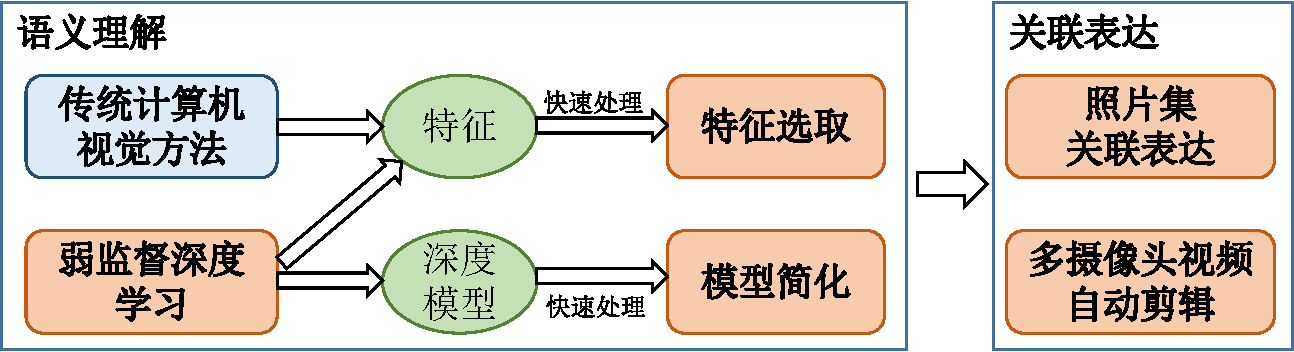
\includegraphics[width=0.9\textwidth]{correlation.pdf}
\caption{社交多媒体数据的研究内容和相互关联}
\label{fig:correlation}
\note{橙色部分表示本文的研究工作}
\end{figure}

基于以上研究点,本论文具体的研究内容包括:
\begin{enumerate}[{(1)}]
    \item 社交多媒体数据弱监督深度学习的算法研究: 针对任意的图像类别,
        从互联网抓取弱标注数据,提出具有抗噪效果的图片分类模型。
        传统深度学习算法对于噪声的敏感性是由于所有的数据在学习过程中具有相同的权重。
        本论文提出的方法的基本假设是:同一类别下,正确标注的图片由于语义上关联,
        在特征空间上比较接近,而错误标注的图片则与其他图片有很大的差异性。
        因此,我们可以利用图片在特征空间上的关系,
        使得不同的训练数据在训练过程中有不同的贡献加权,
        从而使得在特征空间上“孤立”的图片具有较小的权重,
        特征空间上密集区域的图片具有较大的权重,我们称之为相关反馈。
        该思想可以通过在学习中进行特征空间的低秩分解实现。
        为了加速模型训练的速度,我们进一步通过一系列的推导和近似,
        最终降低模型的复杂度,用于大规模社交多媒体数据的模型训练。

    \item 大规模高维特征选取算法研究:
        多媒体数据特征表述不仅包括高层次的卷积神经网络特征,
        还包含低层次全局特征(如颜色特征,纹理特征),局部特征(如SIFT,SURF)
        以及用来通过局部特征描述整体视觉信息的词袋特征等。
        实际应用中需要根据需求选取对目标任务最有用的特征子集,
        这对于大规模社交多媒体数据的处理速度以及移动设备有限的计算能力和内存空间尤其重要。
        此外,去除特定任务不相干的特征,还可以提高特征的表达能力。
        本论文提出从大规模高维数据中选取特征的高效算法。
        已有稀疏在线特征选取算法的复杂度与特征的维度成正比,
        本论文利用二阶在线学习算法,基于特征的置信度进行特征选择,
        并利用最大最小堆结构提出快速特征选取算法。
        由于置信度的单调递减特性,本文进一步提出了快速二阶在线特征选择算法,
        将算法的复杂度降为与非零特征数目成正比。

    \item 深度学习模型简化算法研究:
        深度卷积神经网络的深度和模型参数通常比较大,
        例如经典的VGG-16网络包含超过200M的模型参数。
        大量的模型参数意味着在实际应用中需要大量的计算资源和时间,
        极大地限制了深度神经网络在大规模图片检索和图片识别等任务上的应用。
        此外,深度网络在移动设备上的应用已经成为一种趋势。由于移动设备计算能力的限制,
        在不影响模型准确度的条件下简化深度网络模型已经成为迫切的需要。
        本论文提出一种基于在线特征选取的模型简化算法。算法主要针对卷积层进行简化,
        对每一个卷积层增加一个卷积核的权重层。
        初始条件下所有卷积核的权重为1,在学习过程中对权重进行更新,
        每次更新后利用稀疏在线特征选取算法将部分权重设为0,保留剩余的权重。
        区别传统方法,稀疏在线学习的方法可以在训练过程中动态的调整需要保留的卷积核,
        从而减小模型简化对模型参数的影响。

    \item 照片集关联表达算法研究:
        照片集的关联表达首先对照片集进行事件检测,找出用户所拍摄的不同事件。
        其次,利用弱监督的深度学习算法进行照片的内容分析和模型简化。
        由于深度网络的每一层都是对照片不同层次的语义表达,
        本文将这些特征拼接到一起组成高维特征,
        并利用本文提出的在线特征选取算法选取最能鉴别照片语义的特征子集,
        构成照片内容的最终表达。为了达到更好的表达效果,
        不同风格的照片需要采用不同的编辑技巧。
        本文设计了17个设计风格,并利用弱监督深度神经网络从网络上抓取训练图片,
        得到设计风格的分类器,将照片集中的事件分配到不同的风格中。
        最后,通过可计算的视频编辑语法,对照片进行动画特效处理以及音乐的匹配,
        最终生成具有关联表达能力的视频呈现给用户。

    \item 移动多摄像头视频自动剪辑算法研究:
        多摄像头视频是指在同一时间段,
        同一地点由不同摄像头拍摄的时间上有重叠的一组视频。
        多摄像头视频是不同的人从不同的角度对相同事件的记录。
        本文提出一个全自动的移动多摄像头视频自动剪辑系统。
        我们首先邀请专业的视频编辑人员探讨可计算的视频编辑语法。
        根据这些语法,自动剪辑系统首先对音频流进行质量评估,
        在保证尽可能减少音频流切换次数的条件下选取高质量的音频流,
        形成最终的单一音频流。对于视频流,首先将多摄像头视频进行语义分割,
        得到视频子镜头,其次对这些子镜头的视觉质量,运动,
        以及相互之间的多样性进行评估,最终在保证镜头运动一致性的前提下,
        最大化质量和多样性,选取视频镜头。对于镜头切换时机的选取,
        则根据音频的节奏以及语义特性,对切换频率进行匹配。
        系统最后将单一的音频流和单一的视频流进行混流,得到最终剪辑好的视频呈现给用户。
\end{enumerate}

\section{本文的主要创新点}
本论文的主要创新点有以下几点:
\begin{itemize}
    \item 针对社交多媒体数据标准难的问题,
        提出一种可以从互联网数据中学习图像类别的深度神经网络学习算法,
        摆脱了对大量标注数据的依赖。该算法利用数据本身之间的关联,
        使得不同的数据在模型训练中有不同的贡献加权。
        同时,通过一系列的推导和简化,最终的模型复杂度低,对于训练大量数据有重要意义。

    \item 针对大规模社交多媒体数据处理慢的问题,
        提出了从大规模高维数据中选取特征的高效算法。
        相比于已有的批处理算法和在线学习算法,该算法大大降低了特征选择的时间复杂度,
        同时,选取的特征具有和传统算法选出的特征差别不大甚至更好的表述能力。

    \item 针对深度模型处理慢,耗费计算资源的问题,
        提出了简化深度卷积神经网络的高效算法,将传统的多维数据组稀疏问题转化为
        经典的一维特征选取问题,在不影响模型准确率的情况下极大减少了模型参数。

    \item 提出了全新的照片集关联表达算法——Monet,
        从个人照片集中自动检测事件,选取有代表意义的图片,
        选取合适的视频编辑风格,并将设计师设计的视频编辑语法应用到照片集的编辑中。

    \item 提出移动多摄像头视频自动剪辑系统——MoVieUp,
        自动编辑移动多摄像头视频并生成一段综合音频视频流的方法。
        该方法首次考虑了音频流的剪辑,
        并且首次系统的讨论视频编辑理论在自动化方法中的应用。
\end{itemize}

\section{本文的结构安排}
本论文主要研究社交多媒体数据的语义理解和关联表达中的几个关键问题:弱监督深度学习,
特征提取,模型简化,以及照片集关联表达和移动多摄像头自动剪辑。各章节内容安排如下:
\begin{itemize}
    \item 第2章从弱监督学习,特征提取,模型简化,
        和关联表达四个方面介绍本论文相关工作的研究现状和工作基础。
        在弱监督学习方面,主要介绍了传统的弱监督学习方法和
        近年来热点研究的弱监督深度学习方法;在特征提取方面,主要回顾了传统的
        批处理方法,用于解决大规模流数据的在线学习方法,和在线特征提取算法;
        在模型简化方面,主要介绍与深度卷积神经网络相关的模型简化工作;
        在关联表达方面,主要介绍学术界和工业界关于社交多媒体数据的研究和代表性应用产品。
    \item 第3章重点介绍弱监督深度相关反馈网络的具体设计思路和实现方法,
        简化模型训练的理论证明和近似策略,以及相应的实验结果。

    \item 第4章介绍大规模社交多美数据快速处理的方法。
        首先介绍在线稀疏学习方法的基本模型,并介绍本文提出的
        置信度加权在线稀疏学习和置信度加权在线特征选取方法。
        本文从大规模标准数据集上验证算法的有效性,
        并在图片检索的实际任务中验证算法的可行性。
        其次,该部分介绍了深度学习模型简化的问题建模和具体算法,
        以及相应的实验结果。

    \item 第5章介绍照片集关联表达系统,包括照片集中事件检测方法,代表性图片选取
        算法及相应的质量评估,多样性评价,和时间均衡性考量。在选取的代表性图片上,
        系统基于弱监督学习算法设计了不同风格的分类器,将照片集中的事件分配到不同的
        风格中,利用针对不同风格设计的可计算的编辑语法,对照片赋予丰富的特效,生成
        具有表现力的视频,重现照片集中的场景和故事。

    \item 第6章介绍移动多摄像头自动剪辑系统。系统首先介绍针对移动多摄像头视频
        自动剪辑的可计算的视频编辑语法,并提出相应的系统框架。该部分详细介绍了
        音频的质量评估和剪辑方法,基于音频节奏和语义内容的视频切换点检测算法
        和基于镜头质量,多样性,和运动连续性的镜头选取算法。最后,通过实验证明
        了系统各个部分的有效性和整体的用户体验。

    \item 第7章对全文进行总结,以及未来可以进一步开展或改进的工作。
\end{itemize}
